\documentclass[../main.tex]{subfiles}
\setlength{\parindent}{10pt}

\begin{document}
\subsection{Experiment}


\subsubsection{Experimental Procedure \& Apparatus}
\noindent The MEG data were recorded using a MEGIN Triux system housed in a magnetically shielded room (MSR; Vacuumschmelze GmbH \& co., Hanau, Germany). Neuromagnetic signals were acquired from  204 orthogonal planar gradiometers and 102 magnetometers at 102 sensor positions.  Horizontal and vertical EOG, the cardiac ECG signals, stimulus markers as well as luminance changes recorded by a photodiode (see below) were acquired together with the  neuromagnetic signal. The data were lowpass filtered online at 330 Hz and sampled at 1000 Hz. Structural magnetic resonance images (MRIs), for later co-registration with the MEG data, were acquired using a 3 Tesla Siemens MAGNETOM Prisma whole-body scanner (Siemens AG, Muenchen, Germany), TE = 2 ms, and TR = 2 s). For two subjects, the T1-weighted images obtained in previous experiments, using a 3 Tesla Philips Achieva Scanner (Philips North America Corporation, Andover, USA), were used (scanned at the former Birmingham University Imaging Centre).  Participants were invited to two separate sessions during which the MEG data and  the anatomical images were acquired, respectively. Whenever possible, the MEG recording preceded the MRI scan; otherwise, the MEG session was scheduled at least 48 hours after the MRI session to avoid any residual magnetisation from the MRI system. Volunteers were requested to remove all metal items (e.g. jewellery) before entering the MSR. To enable later co-registration between MRI and MEG data, four to five head-position-indicator (HPI) coils were attached to the participants' foreheads. Along with the position of the coils, three fiducial landmarks (nasion, left and right tragus) and over 200 head-shape samples were digitized using a Polhemus Fastrak (Polhemus, Colchester, USA). Following the preparation, the participants were seated in upright position under the dewar, with orientation set to 60$^{\circ}$. The MEG experiment consisted of fifteen blocks lasting 4 min 30 s each. Participants were offered breaks every $\sim$20 min but remained seated. At the beginning of each of these recording blocks, subjects were instructed to sit with the top and backside of their head touching the sensor helmet. 
The positions of the HPI coils relative to the sensors was gathered at the beginning of each recording block, but not continuously. The MEG experiment lasted $\sim$75 min in total.

\subsubsection{Rapid photic stimulation} \noindent
Stimuli were presented using a Propixx lite projector (VPixx Technologies Inc, Saint-Bruno, QC Canada) which allows refresh rates of up to 1440 Hz. To achieve this high-frequency mode, the projector separates the screen (initial resolution: $1920\times1080$ pixels) into quadrants and treats them as separate frames, resulting in a display resolution of $960\times540$ pixels. The RGB colour codes for each quadrant, viz. red, green and blue, are converted to a greyscale, separately for each frame and colour, and presented consecutively within one refresh interval. The twelve frames are presented at a refresh rate of 120 Hz, resulting in 12$\times$120 Hz = 1440 Hz. This approach allows to drive the luminance of each pixel with high temporal precision, allowing for smooth sinusoidal modulations, reducing unwanted harmonics (see Figure \ref{fig:paradigm}C,D). In this study, we applied rapid rhythmic stimulation at frequencies ranging from 52 to 90 Hz in 2 Hz increments.

\subsubsection{Experimental Paradigm} \noindent
Stimuli were created in MATLAB 2017a (The MathWorks, Inc. Natick, MA, USA) and presented using the Psychophysics Toolbox Version 3 \citep{brainard1997psychophysics}.
\paragraph{Conditions} The experiment consisted of two conditions that will be referred to as the \RFTonly and the \gammaRFT condition, respectively. Each trial began with a one-second interval, in which a central white fixation cross was presented on a dark grey background. In the \RFTonly trials, a circular patch of size 2.43$^{\circ}$ was presented for 2 s. Its luminance was modulated sinusoidally at frequencies between 52 and 90 Hz (Figure \ref{fig:paradigm}A). Frequencies were randomised and balanced across trials. The patch was centred on the fixation cross, such that it was presented both foveally and parafoveally. To minimise the visibility of the flicker, the mean luminance of the patch was matched to the background (33\% luminance, RGB [84 84 84]). Each trial ended with a two-second interval in which only the fixation cross was presented. In the \gammaRFT condition, the baseline interval was followed by a 2 s presentation of a moving grating stimulus that has been shown to reliably elicit gamma oscillations in visual cortex \citep[e.g.][]{hoogenboom2006localizing,hoogenboom2010visually,muthukumaraswamy2013visual,tan2016meg}. The stimulus was the same size as the patch (2.43$^{\circ}$) and had a spatial frequency of 10.3 cycles/$^{\circ}$ (see Figure \ref{fig:paradigm}B). \textcolor{red}{The rings contracted towards the centre of the screen with a velocity of 0.56 $^{\circ}$/s, i.e. 4 cycles/s.} In the subsequent 2 s interval, the stimulus was flickered at the respective frequencies, followed by another 2 s interval in which the concentric moving circles remained on screen without photic stimulation. To keep the overall brightness of the stimulation similar between conditions, the luminance of the circular patch in the \RFTonly condition ranged from 0 to 66\% (of the projector's maximum), while the brightness of the gratings in the \gammaRFT ranged from 33 and 99\%. \textcolor{red}{The resulting contrast between the grey and black rings, of 66\%, has been previously demonstrated to induce clearly identifiable gamma oscillations \citep{self2016effects}. The range of the photic drive, i.e. the difference between peak and trough, estimated based on the projector's maximum luminance, was 339 lumens.} The flicker was applied to a small circular patch in the lower right corner of the screen, to acquire the stimulation signal with a photodiode. \textcolor{red}{Including both the \RFTonly and \gammaRFT condition enabled us to investigate any differences in the resonance properties of the visual system when set into gamma mode compared to mere stimulation with an almost invisible flicker. Given the filter properties of the visual system \citep[see][for review]{cormack2005computational}, we were further interested in identifying an upper limit of the frequencies inducing reliable responses. As we expect these results to guide future studies employing the rapid flicker for frequency tagging, we chose an invisible patch to avoid any confounds by response enhancement, e.g. by object-based attention or figure-ground segregation \citep{self2016effects}.} 

 \paragraph{Task \& Time Course}
Participants were kept vigilant by performing a simple visual detection task that required them to respond to a 45$^{\circ}$ rotation of the fixation cross at the centre of the screen, which occurred once every minute \citep[e.g.][]{zaehle2010transcranial}. Data including the target and/or the responses were discarded and not considered in the analysis. The rotation took place after a trial in the majority, i.e. 60\%, of the cases. The remaining 40\% of rotations took place at any point during a trial. The experiment was divided into 15 blocks of 4.5 min, resulting in a recording time of 75 min in total. \textcolor{red}{The 40 frequency$\times$condition combinations were presented once in each block, in randomised order, resulting in a total of 15 trials per flicker frequency and condition.} To minimise the amount of trials rejected by eye-blink artefacts, 3 s breaks, indicated by a motivating catchphrase or happy face on the screen, were incorporated every five trials, i.e. every 25 - 35 seconds. Participants were instructed to utilise these breaks to rest their eyes.
\begin{figure}[H]
    \centering
    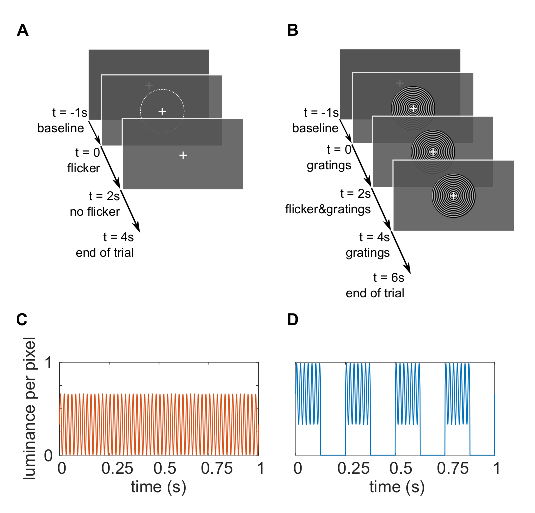
\includegraphics[width=85mm]{figures/fig1_paradigm.eps}
          \captionsetup{width=85mm}

    \caption[Experimental paradigm]{The experimental paradigm. \textbf{A} Trials in the \RFTonly condition. A 1 s baseline interval with a central fixation cross was followed by a 2 s interval of the rapid flicker applied to circular patch of size 2.43$^{\circ}$. The average luminance in the flickering patch was equal to the surrounding grey colour, making the flickering patch almost unperceivable. The trials ended with 2 s of the fixation cross only. \textbf{B} The trials in the \gammaRFT condition. The 1 s baseline interval was followed by 2 s of grating stimuli presented centrally on the screen, contracting inwards. Subsequently, the flicker was imposed onto the stimuli for 2 s. The trial ended with a 2 s presentation of the moving gratings without photic stimulation. \textbf{C} Sinusoidal luminance change in one pixel induced by the photic drive at 52 Hz in the \RFTonly condition. \textbf{D} Luminance change in one pixel as a result of the flicker and the gratings moving concentrically with a velocity of 4 cycles/s. To maintain a similar mean luminance between conditions, photic modulation of the invisible patch in \textbf{A} ranged from 0 to 66\% (mean RGB [84 84 84]), while the light grey rings of the grating, that is 50\% of the stimulus' surface, were flickered between 33 and 99\% (mean RGB [168 168 168] per ring).}
    \label{fig:paradigm}
\end{figure}

\subsubsection{Participants} \noindent
This project was reviewed and approved by the local Ethics Committee at University of Birmingham, UK.
Thirty-one students of the University of Birmingham participated in the experiment. One experimental session was terminated prematurely due to the participant not being cooperative, resulting in a sample of thirty participants (15 female), aged 25.7 $\pm$ 3.4 years. This sample size was decided upon based on a conceptually similar study investigating entrainment of neuronal alpha oscillations by \citet{notbohm2016modification}. All volunteers declared not to have had a history of neuropsychiatric or psychological disorder, reported to be medication-free and had normal or corrected-to-normal vision. For safety reasons, participants with metal items inside their bodies were excluded at the selection state. Prior to  taking part in the study, participants gave informed consent, in accordance with the declaration of Helsinki, to both the MEG recording and the MRI scan and were explicitly apprised of their right to abort the experiment at any point. The reimbursement amounted to \textsterling15 per hour.
To allow analysis of flicker responses at frequencies with a sufficient distance to the individual gamma frequency (IGF; see \ref{IGF}) of the participant, i.e. $\pm$6 Hz, 8 participants were excluded due to their IGF being below 58 Hz. Thus, the data of 22 participants were included in the following analyses (11 female; mean age 25.7 years).

\subsection{Data Analysis}\noindent

Analyses were performed in MATLAB 2017a and 2019b (The MathWorks, Inc. Natick, MA, USA) using the fieldtrip toolbox \citep{oostenveld2011fieldtrip}.

\subsubsection{Sensor Analysis}
At the sensor level, the analysis was confined to the planar gradiometer signals, as these provided the best signal-to-noise ratio. 
\paragraph{MEG preprocessing} Trials containing the target or button presses were excluded. The data were read into MATLAB as 5 s and 7 s trials for the \RFTonly and \gammaRFT conditions, respectively. Artefactual sensors were identified visually during and after the recordings for each participant, and interpolated with the data of their neighbouring sensors (0 to 2 sensors per participant). The individual trials were linearly detrended. Trials containing head movements and/or multiple eye blinks were discarded using a semi-automatic approach. An ICA approach ('runica' implemeted in FieldTrip) was used to project out cardiac signals, eye blinks and eye movement. The sensor positions relative to the HPI coils were loaded in from the data files and averaged for each subject. 
\paragraph{Time-Frequency Representation of Power}
Time-Frequency Representations (TFRs) of power were calculated using a sliding time-window approach ($\Delta$T = 0.5 s; 0.05 s steps). A Hanning taper (0.5 s) was applied prior to the Fourier-transform. This approach induced spectral smoothing of $\pm$3 Hz.  Relative power change in response to the stimulation, i.e. the moving grating and/or the photic drive, was calculated as:

\begin{equation}\label{eq:rlc}
P\textsubscript{normalized} = \frac{P\textsubscript{stim}}{P\textsubscript{base}} - 1   
\end{equation}

with $P\textsubscript{stim}$ being the power during stimulation and $P\textsubscript{base}$ being the power in the baseline interval. The baseline interval was 0.75 - 0.25 s prior to the onset of the flicker (\RFTonly condition) or the moving grating stimulus (\gammaRFT condition).

\paragraph{Individual Gamma Frequency}
The frequency band of the oscillatory activity elicited in response to the moving grating stimulus was identified individually per participant. TFRs of power were calculated for the baseline interval and presentation of the moving grating in the \gammaRFT condition and averaged over trials. The results were averaged over the 0.25 - 1.75 s interval, and the frequency bin with the maximum relative power was considered the Individual Gamma Frequency (IGF). For each participant, the 4 to 6 gradiometers with the strongest gamma response to the moving gratings were selected as the Sensors-of-Interest (SOI).
 
\paragraph{Phase-Locking}
The average phase-synchrony between the photodiode (recording the visual flicker) and the neuromagnetic signal at the SOI was quantified by the Phase-Locking Value (PLV) \citep[][]{lachaux1999measuring,bastos2016tutorial} calculated using a 0.5 s sliding window multiplied with a Hanning taper of equal length. The phases of both signals were calculated from Fourier transformations,  applied to the tapered segments. The PLV was computed separately for each \textit{frequency$\times$condition} combination:

\begin{equation} \label{eq:plv}  PLV = \frac{1}{n}\lvert \sum_{n=1}^{N}exp(j\theta(t,n))\rvert\end{equation}
where $\theta(t,n) = \phi\textsubscript{m}(t,n) - \phi\textsubscript{p}(t,n)$ is the phase difference between the MEG (m) and the photodiode (p) signal at time bin $t$ in trial $n$ \citep[see][p.195 and Figure \ref{fig:freq_fun} and \ref{fig:plat_singlesubj}]{lachaux1999measuring}.  
\paragraph{Phase difference as a measure of entrainment}
Additionally, we investigated changes in phase difference between the photodiode and neuromagnetic signal over time for flicker frequencies of IGF$\pm$6 Hz, to identify intervals of strong synchrony, so-called \textit{phase plateaus}. MEG and photodiode signals ($\Delta$T = 3 cycles = $\frac{3}{f_{flicker}}3/$s) were convolved with a complex Hanning taper using the sliding time window approach. Phase angles were derived from the Fourier transformed time series, unwrapped and subtracted to estimate the phase difference over time for each trial. Plateaus were defined as a constant phase angle (maximum average gradient \< 0.01 rad/ms) over the duration of one cycle of the stimulation frequency:

\begin{equation} \label{eq:plat}   \frac{\sum_{i=1}^{\Delta T}\lvert \nabla\theta_{i}\rvert}{n} \leqslant 0.01 rad/ms\end{equation}

with $\nabla\theta_{i}$ being the gradient, i.e. slope, of the phase angle between MEG and photodiode signal at a given sample $i$; $n$ being the length of the cycle in ms, rounded up to the next integer, e.g. 17 ms for a flicker frequency of 60 Hz. While the PLV quantifies the average phase-similarity of the two signals over trials, this approach \textcolor{red}{is feasible to reveal the intermittency between synchronous and asynchronous phases, which will be smeared by a long sliding window.}

\paragraph{Statistical Analysis} Statistical Analysis was performed in RStudio Version 1.2.1355 (RStudio Inc., Northern Ave, Boston, MA; R version 3.6.1., The R Foundation for Statistical Computing).

\subsubsection{Source Analysis} \noindent
\paragraph{MRI preprocessing} The raw T1 weighted images were converted from DICOM to NIFTI. The coordinate system of the participants' individual MRI was aligned to the anatomical landmarks using the head-surface obtained from the MRI and the scalp shapes digitised prior to the recordings. Realignment was done automatically using the Iterative Closest Point (ICP) algorithm \citep{besl1992method} implemented in the FieldTrip toolbox and corrected manually as necessary. The digitised headshape of one participant, for whom there was no anatomical image available, was aligned to a standardised template brain.
 
\paragraph{Linearly Constrained Minimum Variance Beamforming} The neuroanatomical origins of the visually induced gamma oscillations in the \gammaRFT condition and the response induced by the photic drive in the \RFTonly condition were estimated using Linearly Constrained Minimum Variance spatial filters \citep[LCMV;][]{van1997localization}, implemented in the Fieldtrip Toolbox \citep{oostenveld2011fieldtrip}. The MEG forward model was calculated using single-shell head-models, estimated based on the aligned anatomical images, and an equally spaced 4-mm grid, warped into MNI (Montreal Neurologic Institute) space  \citep[\citealt{nolte2003magnetic}, also see][]{oostenveld2011fieldtrip,stenroos2014comparison}; yielding 37,163 dipoles inside the brain. The pre-processed data, epoched in 7 and 5-second trials for the respective conditions, were band-pass filtered at 50 to 92 Hz, by applying second order Butterworth two-pass high- and low-pass filters. \textcolor{red}{Segments of 0.5 s of the baseline interval (0.75 - 0.25 s prior to stimulation) and stimulation interval (0.75 - 1.25 s after flicker/grating onset, 2.75 - 3.25 to identify the flicker response in \gammaRFT) were extracted from the filtered data}. For each participant, a common covariance matrix for the 204 planar gradiometers was computed based on the extracted time series and used to estimate the spatial filter coefficients for each dipole location, whereby only the direction with the highest dipole moment was considered. Data in the baseline and stimulation intervals were projected to source space by multiplying each filter coefficient with the sensor time series. Fast Fourier Transforms of the resulting time series, multiplied with a Hanning taper, were computed for each of the 37,163 virtual channels, separately for the baseline and stimulation intervals, and averaged over trials. Relative power change at the IGF and flicker frequencies was computed by applying equation \eqref{eq:rlc} to the Fourier-transformed baseline and stimulation intervals. The source-localised power change values at flicker frequencies up to 78 Hz were averaged to identify a common source for the oscillatory response to the photic drive.




\end{document}

